\documentclass[12pt]{article}\usepackage[]{graphicx}\usepackage[]{color}
%% maxwidth is the original width if it is less than linewidth
%% otherwise use linewidth (to make sure the graphics do not exceed the margin)
\makeatletter
\def\maxwidth{ %
  \ifdim\Gin@nat@width>\linewidth
    \linewidth
  \else
    \Gin@nat@width
  \fi
}
\makeatother

\definecolor{fgcolor}{rgb}{0, 0, 0}
\newcommand{\hlnum}[1]{\textcolor[rgb]{0.502,0,0.502}{\textbf{#1}}}%
\newcommand{\hlstr}[1]{\textcolor[rgb]{0.651,0.522,0}{#1}}%
\newcommand{\hlcom}[1]{\textcolor[rgb]{1,0.502,0}{#1}}%
\newcommand{\hlopt}[1]{\textcolor[rgb]{1,0,0.502}{\textbf{#1}}}%
\newcommand{\hlstd}[1]{\textcolor[rgb]{0,0,0}{#1}}%
\newcommand{\hlkwa}[1]{\textcolor[rgb]{0.733,0.475,0.467}{\textbf{#1}}}%
\newcommand{\hlkwb}[1]{\textcolor[rgb]{0.502,0.502,0.753}{\textbf{#1}}}%
\newcommand{\hlkwc}[1]{\textcolor[rgb]{0,0.502,0.753}{#1}}%
\newcommand{\hlkwd}[1]{\textcolor[rgb]{0,0.267,0.4}{#1}}%

\usepackage{framed}
\makeatletter
\newenvironment{kframe}{%
 \def\at@end@of@kframe{}%
 \ifinner\ifhmode%
  \def\at@end@of@kframe{\end{minipage}}%
  \begin{minipage}{\columnwidth}%
 \fi\fi%
 \def\FrameCommand##1{\hskip\@totalleftmargin \hskip-\fboxsep
 \colorbox{shadecolor}{##1}\hskip-\fboxsep
     % There is no \\@totalrightmargin, so:
     \hskip-\linewidth \hskip-\@totalleftmargin \hskip\columnwidth}%
 \MakeFramed {\advance\hsize-\width
   \@totalleftmargin\z@ \linewidth\hsize
   \@setminipage}}%
 {\par\unskip\endMakeFramed%
 \at@end@of@kframe}
\makeatother

\definecolor{shadecolor}{rgb}{.97, .97, .97}
\definecolor{messagecolor}{rgb}{0, 0, 0}
\definecolor{warningcolor}{rgb}{1, 0, 1}
\definecolor{errorcolor}{rgb}{1, 0, 0}
\newenvironment{knitrout}{}{} % an empty environment to be redefined in TeX

\usepackage{alltt}
\usepackage{setspace}
%\documentclass[a4paper,12pt]{article}
\usepackage[utf8]{inputenc}
\usepackage{amsmath}
%\usepackage[brazil,brazilian]{babel}
\usepackage{indentfirst}
\usepackage{graphicx}
\usepackage{color}
\usepackage{graphics}
\setlength{\parindent}{1.0cm}
%\setlength{\textheight}{10.5in}
%\setlength{\textwidth}{6in}
\setlength{\oddsidemargin}{0.1in}
\setlength{\evensidemargin}{0.0in}
\addtolength{\topmargin}{-1.0in}
%\setlength{\parskip}{0.1in}
%\parskip=15pt
%\setlength{\unitlength}{0.01in}
%\usepackage{Sweave}
%\usepackage[pdftex]{hyperref}
\usepackage[bottom=2cm,top=3cm,left=3cm,right=2cm]{geometry}
\usepackage{placeins}
\usepackage{float}
\usepackage{hyperref}


%\pagestyle{empty}

\title{\textbf{Plano Amostral}}
\author{Felipe Barletta}
%\date{}
\IfFileExists{upquote.sty}{\usepackage{upquote}}{}
\begin{document}
\onehalfspacing
\maketitle
\indent
%\pagestyle{headings}



\section{Amostra por domicílios}

\indent

O objetivo do estudo, que é verificar o comportamento acerca do descarte
de resíduos de cozinha adequadamente no bairro de Santa Felicidade em
Curitiba-PR.\\
\indent
Como há uma limitação operacional para a coleta dos dados, optou-se por
simular vários cenários de amostragem para que a pesquisadora adote o mais
viável planejamento amostral dentro de suas condições de aplicação dos
questionários e captação das informações.\\
\indent
O planejamento amostral será realizado com a premissa de uma
amostra por domicílio dentro da região geográfica que abrange a população
alvo da pesquisa.\\
\indent
A população alvo são todos os domicílios residenciais do bairro de Santa
Felicidade em Curitiba-PR. Desta área será coletada a amostra do estudo.\\
\indent
Portanto a unidade amostral será a residência e
a unidade observacional será a pessoa entrevistada(responsável pelo domicílio). \\
\indent
Serão simulados dois cenários:
\begin{itemize}
  \item Amostragem Estratificada
  \item Amostragem aleatória simples sem reposição
\end{itemize}

Em cada cenário, o tamanho da amostra será alocado com diferentes erros amostrais:
\begin{itemize}
  \item 0,03
  \item 0,05
  \item 0,06
  \item 0,08
  \item 0,10
\end{itemize}

\subsection{Estimativa dos parâmetros}
\indent

Por convenção denotamos $N$ para o tamanho populacional e $n$ o tamanho
amostral.\\
\indent
Antes da descrição dos tipos de amostragem usados neste estudo, vamos definir
e estimar os parâmetros de interesse neste estudo, para isso consideraremos
os resultados de uma estudo piloto realizado em um colégio estadual situado
no bairro de Santa Felicidade, sobre o descarte de óleo residual de cozinha.
Na questão $3$ usada para coleta dos dados da amostra piloto, perguntava-se:\\
"\textit{3)  Como sua família descarta o resíduo de óleo após seu uso?}"\\
\indent
Vamos discutir a estimação de uma proporção $P$, ou seja, a proporção de respostas 
da pergunta acima que disseram que armazenam o óleo residual para entrega em ponto 
de coleta. Quem respondeu diferente desta resposta será considerada a
estimativa da proporção complementar, $Q$, ou $1-P$.\\
\indent
Dos 254 questionários que compuseram a amostra piloto, foram excluídos, para
cálculo das estimativas, 60 que responderam "\textit{Não sei}" e 1 que
não respondeu. Dos entrevistados $68$ responderam que separam o óleo
residual para coleta, portanto as estimativas ficaram da seguinte forma:\\

 $$ \hat{P} = 68/184 = 0,37 $$
 $$ \hat{Q} = 1-\hat{P} = 0,63 $$

Utilizando a aproximação de normalidade assintótica teremos o seguinte
intervalo de confiança para a estimativa pontual de $\hat{P}$:\\

\begin{equation}
   IC(\hat{P}) = \left( \hat{P}-z_\alpha \sqrt{(1-f)\frac{\hat{P} \hat{Q}}{n-1}}; \hat{P}+z_\alpha \sqrt{(1-f)\frac{\hat{P} \hat{Q}}{n-1}} \right)
\end{equation}
 Como ainda não sabemos o tamanho da nossa população vamos considerar nosso
 $N$, que se refere ao tamanho populacional, como infinito. Então a fração amostral $f=n/N$
 tenderá a zero. Fazendo os cálculo teremos um intervalo de confiança com
 $95\%$ de confiança igual à:

\indent


$$
IC(\hat{P}) = ( 0.3; 0.44)
$$

%$$
%{\displaystyle z=\left( \frac {e^{i\theta}+e^{-i\theta}}{2}\right)^2 +\left(\frac{e^{i\theta}-e^{-i\theta}}{2i} \right)^2}
%$$

\subsection{Amostragem Estratificada}
\indent

Este será o primeiro cenário para o plano amostral.\\
\indent
A amostragem estratificada consiste na divisão de uma população em grupos ou
estratos segundo alguma característica conhecida na população em estudo.\\
\indent
Neste estudo ela será usada para a melhoria da precisão da estimativa da
proporção de famílias que descartam corretamente o resíduo de cozinha.\\
\indent
Os estratos considerados serão os setores censitários definidos pelo IBGE
no último censo de $2010$,
\url{http://www.censo2010.ibge.gov.br/sinopseporsetores/?nivel=st}.\\
\indent
Dentro de cada estrato será realizada uma amostra aleatória simples sem reposição, 
em que cada domicílio dentro dos estratos têm a mesma chance de ser escolhidos. 
Para cálculo do tamanho da amostra. O bairro de Santa Felicidade possui $38$
setores censitários, portanto teremos 38 estratos, como vemos na figura 1.\\
\indent
A expressão utilizada para determinar o tamanho na amostra, considerando
estratos com população finita, será:\\

\begin{equation}
  n_{h} = \frac{N\hat{P}\hat{Q}Z^{2}}{\hat{P}\hat{Q}Z^{2}+(N+1)E^{2}}
\end{equation}
Em que:\\
\indent

\begin{itemize}
\item $n_h$: tamanho da amostra do estrato \textit{h};
\item Z: Quantil da distribuição (nível de significância) \textit{Normal};
\item E: Erro amostral assumido.
\end{itemize}




\begin{knitrout}\footnotesize
\definecolor{shadecolor}{rgb}{0.902, 0.902, 0.98}\color{fgcolor}\begin{figure}[H]

{\centering 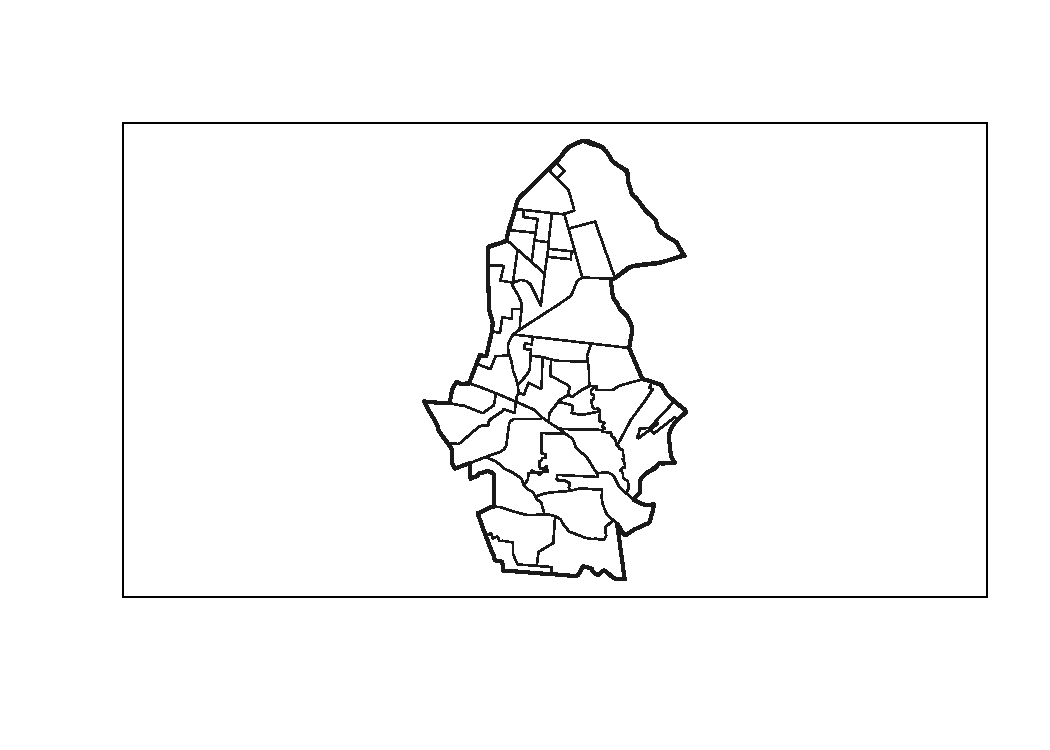
\includegraphics[width=1\linewidth]{figure/plot1-1} 

}

\caption[Bairro de Santa Felicidade 
 por setores censitários]{Bairro de Santa Felicidade 
 por setores censitários}\label{fig:plot1}
\end{figure}


\end{knitrout}
\indent



\subsubsection{Variando erro amostral}
\indent

Cálculo do tamanho da amostra com erro amostral $0,03$, considerando o limite
inferior do intervalo de confiança para $\hat{P}$.
\indent





\begin{knitrout}\footnotesize
\definecolor{shadecolor}{rgb}{0.902, 0.902, 0.98}\color{fgcolor}\begin{kframe}
\begin{verbatim}
  n1  n2  n3  n4  n5  n6  n7  n8  n9 n10 n11 n12 n13 n14 n15 n16 n17 n18
 226 221 267 250 212 172 175 224 226 201 253 234 214 294 231 257 199 317
 n19 n20 n21 n22 n23 n24 n25 n26 n27 n28 n29 n30 n31 n32 n33 n34 n35 n36
 268 184 239 318 193 240 170 156 166 216 229 321 263 345 275 200 209 179
 n37 n38
 149 330
\end{verbatim}
\end{kframe}
\end{knitrout}

Cálculo do tamanho da amostra com erro amostral $0,05$, considerando o limite
inferior do intervalo de confiança para $\hat{P}$.



\begin{knitrout}\footnotesize
\definecolor{shadecolor}{rgb}{0.902, 0.902, 0.98}\color{fgcolor}\begin{kframe}
\begin{verbatim}
  n1  n2  n3  n4  n5  n6  n7  n8  n9 n10 n11 n12 n13 n14 n15 n16 n17 n18
 156 154 175 167 150 129 130 155 156 144 169 160 150 186 159 170 143 195
 n19 n20 n21 n22 n23 n24 n25 n26 n27 n28 n29 n30 n31 n32 n33 n34 n35 n36
 175 135 162 195 140 163 127 119 125 151 158 196 173 205 178 143 148 132
 n37 n38
 115 200
\end{verbatim}
\end{kframe}
\end{knitrout}

Cálculo do tamanho da amostra com erro amostral $0,06$, considerando o limite
inferior do intervalo de confiança para $\hat{P}$.


\begin{knitrout}\footnotesize
\definecolor{shadecolor}{rgb}{0.902, 0.902, 0.98}\color{fgcolor}\begin{kframe}
\begin{verbatim}
  n1  n2  n3  n4  n5  n6  n7  n8  n9 n10 n11 n12 n13 n14 n15 n16 n17 n18
 129 127 141 136 124 109 110 128 129 120 137 132 125 148 130 138 120 154
 n19 n20 n21 n22 n23 n24 n25 n26 n27 n28 n29 n30 n31 n32 n33 n34 n35 n36
 141 114 133 154 117 133 109 103 107 126 130 155 140 160 143 120 123 112
 n37 n38
  99 157
\end{verbatim}
\end{kframe}
\end{knitrout}

Cálculo do tamanho da amostra com erro amostral $0,08$, considerando o limite
inferior do intervalo de confiança para $\hat{P}$.


\begin{knitrout}\footnotesize
\definecolor{shadecolor}{rgb}{0.902, 0.902, 0.98}\color{fgcolor}\begin{kframe}
\begin{verbatim}
 n1 n2 n3 n4 n5 n6 n7 n8 n9 n10 n11 n12 n13 n14 n15 n16 n17 n18 n19 n20
 89 88 95 93 87 79 80 89 89  85  93  90  87  98  90  94  85 100  95  82
 n21 n22 n23 n24 n25 n26 n27 n28 n29 n30 n31 n32 n33 n34 n35 n36 n37 n38
  91 101  83  91  79  76  78  88  90 101  94 103  96  85  86  81  74 102
\end{verbatim}
\end{kframe}
\end{knitrout}

Cálculo do tamanho da amostra com erro amostral $0,10$, considerando o limite
inferior do intervalo de confiança para $\hat{P}$.


\begin{knitrout}\footnotesize
\definecolor{shadecolor}{rgb}{0.902, 0.902, 0.98}\color{fgcolor}\begin{kframe}
\begin{verbatim}
 n1 n2 n3 n4 n5 n6 n7 n8 n9 n10 n11 n12 n13 n14 n15 n16 n17 n18 n19 n20
 64 63 67 66 63 59 59 64 64  62  66  64  63  68  64  66  62  69  67  60
 n21 n22 n23 n24 n25 n26 n27 n28 n29 n30 n31 n32 n33 n34 n35 n36 n37 n38
  65  69  61  65  58  57  58  63  64  70  66  71  67  62  62  60  56  70
\end{verbatim}
\end{kframe}
\end{knitrout}

\subsection{Amostragem Aleatória Simples Sem Reposição}
\indent

A amostragem aleatória simples sem reposição (AASs) opera da seguinte forma e
não há estratos, ou seja, os setores censitários não são considerados:
\begin{itemize}
  \item A população será do bairro será numerada de 1 a $N$;
  \item Todos os elementos da população têm a mesma chance de
    serem sorteados;
  \item Sorteia-se um elemento de forma aleatória;
  \item O próximo elemento é sorteado sendo que o anterior foi
    retirado da população
\end{itemize}

\subsubsection{Variando o erro amostral}
\indent
Primeiro vamos calcular o tamanho da amostra como no cenário anterior,
considerando vários erros amostrais. Sabemos que a população total do
bairro é:\\
\indent

$N = 12174$ domicílios \\
\indent



\begin{knitrout}\footnotesize
\definecolor{shadecolor}{rgb}{0.902, 0.902, 0.98}\color{fgcolor}\begin{kframe}
\begin{verbatim}
             n
Erro(0,03) 835
Erro(0,05) 314
Erro(0,06) 220
Erro(0,08) 125
Erro(0,10)  80
\end{verbatim}
\end{kframe}
\end{knitrout}

\subsubsection{Variando o tamanho da amostra}
\indent

Aqui o tamanho da amostra será fixo e o erro amostral
é calculado com base neste tamanho. Os valores fixos da amostra serão, 100, 300,
500 e 1000.\\

\begin{knitrout}\footnotesize
\definecolor{shadecolor}{rgb}{0.902, 0.902, 0.98}\color{fgcolor}\begin{kframe}
\begin{verbatim}
        Erro
n=100  0.089
n=300  0.051
n=500  0.039
n=1000 0.027
\end{verbatim}
\end{kframe}
\end{knitrout}

\section{Considerações Finais}
\indent

O plano estratificado proporcional produz variâncias sempre menores que aquelas
produzidas por uma amostra aleatória simples (com ou sem reposição) de mesmo
tamanho, e este ganho é maior quanto maior for a variância dos estratos, isto é,
quanto maior for a diferença entre as estimativas dos parâmetros dos estratos.
Os cálculos das variâncias foram omitidas neste trabalho mas o conhecimento
destes fatos é importante para o estatístico desenhar um plano amostral mais
conveniente de acordo com a possibilidade de aplicação dos pesquisadores.

\begin{thebibliography}{99}

\bibitem{bryer2013likert} Bolfarine, H and Bussab, W.
\emph{Elementos de Amostragem}.
Editora Blucher-(2005).


\bibitem{R} R Core Team (2016).
\emph{R: A language and environment for statistical computing. R Foundation for
  Statistical Computing}.
Viena, Austria. \url{http://www.R-project.org/}.

\bibitem{IBGE1} \url{http://www.censo2010.ibge.gov.br/sinopseporsetores/?nivel=st}.

\bibitem{IBGE1} \url{http://www.censo2010.ibge.gov.br/cnefe/}.

\end{thebibliography}

\end{document}
